% Options for packages loaded elsewhere
\PassOptionsToPackage{unicode}{hyperref}
\PassOptionsToPackage{hyphens}{url}
\PassOptionsToPackage{dvipsnames,svgnames,x11names}{xcolor}
%
\documentclass[
  letterpaper,
  DIV=11,
  numbers=noendperiod]{scrartcl}

\usepackage{amsmath,amssymb}
\usepackage{iftex}
\ifPDFTeX
  \usepackage[T1]{fontenc}
  \usepackage[utf8]{inputenc}
  \usepackage{textcomp} % provide euro and other symbols
\else % if luatex or xetex
  \usepackage{unicode-math}
  \defaultfontfeatures{Scale=MatchLowercase}
  \defaultfontfeatures[\rmfamily]{Ligatures=TeX,Scale=1}
\fi
\usepackage{lmodern}
\ifPDFTeX\else  
    % xetex/luatex font selection
\fi
% Use upquote if available, for straight quotes in verbatim environments
\IfFileExists{upquote.sty}{\usepackage{upquote}}{}
\IfFileExists{microtype.sty}{% use microtype if available
  \usepackage[]{microtype}
  \UseMicrotypeSet[protrusion]{basicmath} % disable protrusion for tt fonts
}{}
\makeatletter
\@ifundefined{KOMAClassName}{% if non-KOMA class
  \IfFileExists{parskip.sty}{%
    \usepackage{parskip}
  }{% else
    \setlength{\parindent}{0pt}
    \setlength{\parskip}{6pt plus 2pt minus 1pt}}
}{% if KOMA class
  \KOMAoptions{parskip=half}}
\makeatother
\usepackage{xcolor}
\setlength{\emergencystretch}{3em} % prevent overfull lines
\setcounter{secnumdepth}{-\maxdimen} % remove section numbering
% Make \paragraph and \subparagraph free-standing
\ifx\paragraph\undefined\else
  \let\oldparagraph\paragraph
  \renewcommand{\paragraph}[1]{\oldparagraph{#1}\mbox{}}
\fi
\ifx\subparagraph\undefined\else
  \let\oldsubparagraph\subparagraph
  \renewcommand{\subparagraph}[1]{\oldsubparagraph{#1}\mbox{}}
\fi

\usepackage{color}
\usepackage{fancyvrb}
\newcommand{\VerbBar}{|}
\newcommand{\VERB}{\Verb[commandchars=\\\{\}]}
\DefineVerbatimEnvironment{Highlighting}{Verbatim}{commandchars=\\\{\}}
% Add ',fontsize=\small' for more characters per line
\newenvironment{Shaded}{}{}
\newcommand{\AlertTok}[1]{\textcolor[rgb]{0.16,0.16,0.16}{\textbf{\colorbox[rgb]{0.80,0.14,0.11}{#1}}}}
\newcommand{\AnnotationTok}[1]{\textcolor[rgb]{0.60,0.59,0.10}{#1}}
\newcommand{\AttributeTok}[1]{\textcolor[rgb]{0.84,0.60,0.13}{#1}}
\newcommand{\BaseNTok}[1]{\textcolor[rgb]{0.96,0.45,0.00}{#1}}
\newcommand{\BuiltInTok}[1]{\textcolor[rgb]{0.84,0.36,0.05}{#1}}
\newcommand{\CharTok}[1]{\textcolor[rgb]{0.69,0.38,0.53}{#1}}
\newcommand{\CommentTok}[1]{\textcolor[rgb]{0.57,0.51,0.45}{#1}}
\newcommand{\CommentVarTok}[1]{\textcolor[rgb]{0.57,0.51,0.45}{#1}}
\newcommand{\ConstantTok}[1]{\textcolor[rgb]{0.69,0.38,0.53}{\textbf{#1}}}
\newcommand{\ControlFlowTok}[1]{\textcolor[rgb]{0.80,0.14,0.11}{\textbf{#1}}}
\newcommand{\DataTypeTok}[1]{\textcolor[rgb]{0.84,0.60,0.13}{#1}}
\newcommand{\DecValTok}[1]{\textcolor[rgb]{0.96,0.45,0.00}{#1}}
\newcommand{\DocumentationTok}[1]{\textcolor[rgb]{0.60,0.59,0.10}{#1}}
\newcommand{\ErrorTok}[1]{\textcolor[rgb]{0.80,0.14,0.11}{\underline{#1}}}
\newcommand{\ExtensionTok}[1]{\textcolor[rgb]{0.41,0.62,0.42}{\textbf{#1}}}
\newcommand{\FloatTok}[1]{\textcolor[rgb]{0.96,0.45,0.00}{#1}}
\newcommand{\FunctionTok}[1]{\textcolor[rgb]{0.41,0.62,0.42}{#1}}
\newcommand{\ImportTok}[1]{\textcolor[rgb]{0.41,0.62,0.42}{#1}}
\newcommand{\InformationTok}[1]{\textcolor[rgb]{0.16,0.16,0.16}{\colorbox[rgb]{0.51,0.65,0.60}{#1}}}
\newcommand{\KeywordTok}[1]{\textcolor[rgb]{0.24,0.22,0.21}{\textbf{#1}}}
\newcommand{\NormalTok}[1]{\textcolor[rgb]{0.24,0.22,0.21}{#1}}
\newcommand{\OperatorTok}[1]{\textcolor[rgb]{0.24,0.22,0.21}{#1}}
\newcommand{\OtherTok}[1]{\textcolor[rgb]{0.41,0.62,0.42}{#1}}
\newcommand{\PreprocessorTok}[1]{\textcolor[rgb]{0.84,0.36,0.05}{#1}}
\newcommand{\RegionMarkerTok}[1]{\textcolor[rgb]{0.57,0.51,0.45}{\colorbox[rgb]{0.98,0.96,0.84}{#1}}}
\newcommand{\SpecialCharTok}[1]{\textcolor[rgb]{0.69,0.38,0.53}{#1}}
\newcommand{\SpecialStringTok}[1]{\textcolor[rgb]{0.60,0.59,0.10}{#1}}
\newcommand{\StringTok}[1]{\textcolor[rgb]{0.60,0.59,0.10}{#1}}
\newcommand{\VariableTok}[1]{\textcolor[rgb]{0.27,0.52,0.53}{#1}}
\newcommand{\VerbatimStringTok}[1]{\textcolor[rgb]{0.60,0.59,0.10}{#1}}
\newcommand{\WarningTok}[1]{\textcolor[rgb]{0.16,0.16,0.16}{\colorbox[rgb]{0.98,0.74,0.18}{#1}}}

\providecommand{\tightlist}{%
  \setlength{\itemsep}{0pt}\setlength{\parskip}{0pt}}\usepackage{longtable,booktabs,array}
\usepackage{calc} % for calculating minipage widths
% Correct order of tables after \paragraph or \subparagraph
\usepackage{etoolbox}
\makeatletter
\patchcmd\longtable{\par}{\if@noskipsec\mbox{}\fi\par}{}{}
\makeatother
% Allow footnotes in longtable head/foot
\IfFileExists{footnotehyper.sty}{\usepackage{footnotehyper}}{\usepackage{footnote}}
\makesavenoteenv{longtable}
\usepackage{graphicx}
\makeatletter
\def\maxwidth{\ifdim\Gin@nat@width>\linewidth\linewidth\else\Gin@nat@width\fi}
\def\maxheight{\ifdim\Gin@nat@height>\textheight\textheight\else\Gin@nat@height\fi}
\makeatother
% Scale images if necessary, so that they will not overflow the page
% margins by default, and it is still possible to overwrite the defaults
% using explicit options in \includegraphics[width, height, ...]{}
\setkeys{Gin}{width=\maxwidth,height=\maxheight,keepaspectratio}
% Set default figure placement to htbp
\makeatletter
\def\fps@figure{htbp}
\makeatother

% load packages
\usepackage{geometry}
\usepackage{xcolor}
\usepackage{eso-pic}
\usepackage{fancyhdr}
\usepackage{sectsty}
\usepackage{fontspec}
\usepackage{titlesec}
\usepackage{listings} % For code listings

%% Set page size with a wider right margin
\geometry{a4paper, total={170mm,257mm}, left=20mm, top=20mm, bottom=20mm, right=50mm}

%% Define colors
\definecolor{light}{HTML}{D73F09}
\definecolor{highlight}{HTML}{800080}
\definecolor{dark}{HTML}{330033}

%% Let's add the border on the right hand side 
\AddToShipoutPicture{% 
    \AtPageLowerLeft{% 
        \put(\LenToUnit{\dimexpr\paperwidth-3cm},0){% 
            \color{light}\rule{3cm}{\LenToUnit\paperheight}%
          }%
     }%
     % logo
    \AtPageLowerLeft{% start the bar at the bottom right of the page
        \put(\LenToUnit{\dimexpr\paperwidth-3.95cm},26cm){% move it to the top right
            \color{light}
\includegraphics[width=5cm]{_extensions/nrennie/PrettyPDF/logo.png}
          }%
     }%
}

%% Style the page number
\fancypagestyle{mystyle}{
  \fancyhf{}
  \renewcommand\headrulewidth{0pt}
  \fancyfoot[R]{\fontsize{28}{12}\selectfont\thepage} % Increase the font size by 10pt
  \fancyfootoffset{3.65cm}
}
\setlength{\footskip}{20pt}

%% style the chapter/section fonts
\chapterfont{\color{dark}\fontsize{20}{16.8}\selectfont}
\sectionfont{\color{dark}\fontsize{20}{16.8}\selectfont}
\subsectionfont{\color{dark}\fontsize{14}{16.8}\selectfont}
\titleformat{\subsection}
  {\sffamily\Large\bfseries}{\thesection}{1em}{}[{\titlerule[0.8pt]}]
  
% left align title
\makeatletter
\renewcommand{\maketitle}{\bgroup\setlength{\parindent}{0pt}
\begin{flushleft}
  {\sffamily\huge\textbf{\MakeUppercase{\@title}}} \vspace{0.3cm} \newline
  {\Large {\@subtitle}} \newline
  {\large\@author} \newline
  {\large\today} % Include the full date here
\end{flushleft}\egroup
}
\makeatother


%% Use some custom fonts
\setsansfont{Georgia}[
    Path=_extensions/nrennie/PrettyPDF/Georgia/,
    Scale=0.9,
    Extension = .ttf,
    UprightFont=*,
    BoldFont=*b,
    ItalicFont=*i,
    ]

\setmainfont{Kievit}[
    Path=_extensions/nrennie/PrettyPDF/Kievit/,
    Scale=0.9,
    Extension = .ttf,
    UprightFont=* Regular,
    BoldFont=* Bold,
    ItalicFont=* Black Italic,
    ]
\KOMAoption{captions}{tableheading}
\makeatletter
\makeatother
\makeatletter
\makeatother
\makeatletter
\@ifpackageloaded{caption}{}{\usepackage{caption}}
\AtBeginDocument{%
\ifdefined\contentsname
  \renewcommand*\contentsname{Table of contents}
\else
  \newcommand\contentsname{Table of contents}
\fi
\ifdefined\listfigurename
  \renewcommand*\listfigurename{List of Figures}
\else
  \newcommand\listfigurename{List of Figures}
\fi
\ifdefined\listtablename
  \renewcommand*\listtablename{List of Tables}
\else
  \newcommand\listtablename{List of Tables}
\fi
\ifdefined\figurename
  \renewcommand*\figurename{Figure}
\else
  \newcommand\figurename{Figure}
\fi
\ifdefined\tablename
  \renewcommand*\tablename{Table}
\else
  \newcommand\tablename{Table}
\fi
}
\@ifpackageloaded{float}{}{\usepackage{float}}
\floatstyle{ruled}
\@ifundefined{c@chapter}{\newfloat{codelisting}{h}{lop}}{\newfloat{codelisting}{h}{lop}[chapter]}
\floatname{codelisting}{Listing}
\newcommand*\listoflistings{\listof{codelisting}{List of Listings}}
\makeatother
\makeatletter
\@ifpackageloaded{caption}{}{\usepackage{caption}}
\@ifpackageloaded{subcaption}{}{\usepackage{subcaption}}
\makeatother
\makeatletter
\@ifpackageloaded{tcolorbox}{}{\usepackage[skins,breakable]{tcolorbox}}
\makeatother
\makeatletter
\@ifundefined{shadecolor}{\definecolor{shadecolor}{HTML}{000000}}
\makeatother
\makeatletter
\makeatother
\makeatletter
\makeatother
\ifLuaTeX
  \usepackage{selnolig}  % disable illegal ligatures
\fi
\IfFileExists{bookmark.sty}{\usepackage{bookmark}}{\usepackage{hyperref}}
\IfFileExists{xurl.sty}{\usepackage{xurl}}{} % add URL line breaks if available
\urlstyle{same} % disable monospaced font for URLs
\hypersetup{
  pdftitle={ST557: Homework 5},
  pdfauthor={Brian Cervantes Alvarez},
  colorlinks=true,
  linkcolor={highlight},
  filecolor={Maroon},
  citecolor={Blue},
  urlcolor={highlight},
  pdfcreator={LaTeX via pandoc}}

\title{ST557: Homework 5}
\author{Brian Cervantes Alvarez}
\date{2023-11-30}

\begin{document}
\maketitle
\pagestyle{mystyle}

\ifdefined\Shaded\renewenvironment{Shaded}{\begin{tcolorbox}[interior hidden, boxrule=0pt, borderline west={3pt}{0pt}{shadecolor}, enhanced, sharp corners, breakable, frame hidden]}{\end{tcolorbox}}\fi

\hypertarget{question-1}{%
\section{Question 1}\label{question-1}}

\hypertarget{part-a}{%
\subsection{Part A}\label{part-a}}

\begin{Shaded}
\begin{Highlighting}[]
\CommentTok{\# Load required libraries}
\FunctionTok{library}\NormalTok{(cluster)}

\CommentTok{\# Read the data from TrackData.csv}
\NormalTok{trackData }\OtherTok{\textless{}{-}} \FunctionTok{read.csv}\NormalTok{(}\StringTok{"TrackData.csv"}\NormalTok{)}

\CommentTok{\# Extract numeric columns (excluding the country names and abbreviations)}
\NormalTok{numericData }\OtherTok{\textless{}{-}}\NormalTok{ trackData[, }\SpecialCharTok{{-}}\FunctionTok{c}\NormalTok{(}\DecValTok{1}\NormalTok{, }\DecValTok{2}\NormalTok{)]}

\CommentTok{\# Function to calculate Euclidean distances between countries}
\NormalTok{euclideanDistances }\OtherTok{\textless{}{-}} \FunctionTok{dist}\NormalTok{(numericData, }\AttributeTok{method =} \StringTok{"euclidean"}\NormalTok{)}

\CommentTok{\# Part 1: Hierarchical clustering using single and complete linkage}
\NormalTok{singleLinkageClusters }\OtherTok{\textless{}{-}} \FunctionTok{hclust}\NormalTok{(euclideanDistances, }\AttributeTok{method =} \StringTok{"single"}\NormalTok{)}
\NormalTok{completeLinkageClusters }\OtherTok{\textless{}{-}} \FunctionTok{hclust}\NormalTok{(euclideanDistances, }\AttributeTok{method =} \StringTok{"complete"}\NormalTok{)}

\CommentTok{\# Plot dendrograms}
\FunctionTok{par}\NormalTok{(}\AttributeTok{mfrow =} \FunctionTok{c}\NormalTok{(}\DecValTok{1}\NormalTok{, }\DecValTok{2}\NormalTok{))}
\FunctionTok{plot}\NormalTok{(singleLinkageClusters, }\AttributeTok{main =} \StringTok{"Single Linkage Dendrogram"}\NormalTok{, }\AttributeTok{xlab =} \StringTok{"Countries"}\NormalTok{, }\AttributeTok{sub =} \StringTok{""}\NormalTok{)}
\FunctionTok{plot}\NormalTok{(completeLinkageClusters, }\AttributeTok{main =} \StringTok{"Complete Linkage Dendrogram"}\NormalTok{, }\AttributeTok{xlab =} \StringTok{"Countries"}\NormalTok{, }\AttributeTok{sub =} \StringTok{""}\NormalTok{)}
\end{Highlighting}
\end{Shaded}

\begin{figure}[H]

{\centering 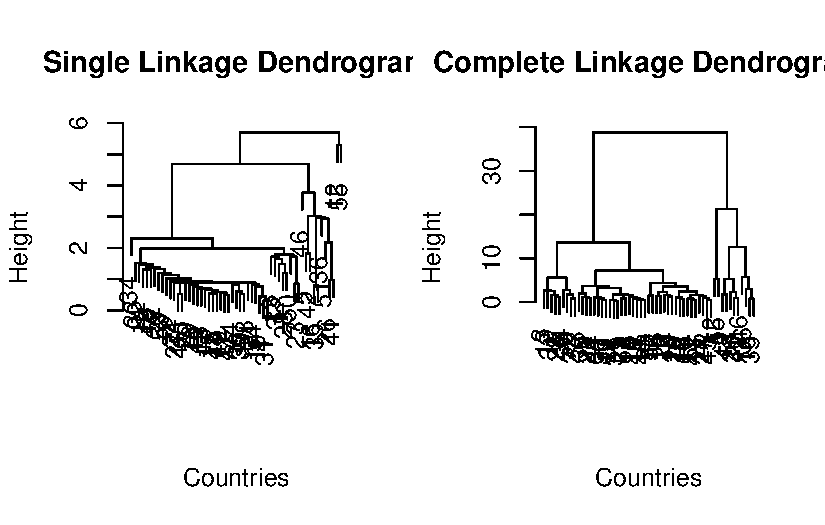
\includegraphics{CervantesAlvarez_Brian_HW5_ST557_files/figure-pdf/unnamed-chunk-1-1.pdf}

}

\end{figure}

\hypertarget{part-b}{%
\subsection{Part B}\label{part-b}}

\begin{Shaded}
\begin{Highlighting}[]
\CommentTok{\# Part 2: Perform k{-}means clustering for k = 2, 3, and 4}
\NormalTok{kMeans2 }\OtherTok{\textless{}{-}} \FunctionTok{kmeans}\NormalTok{(numericData, }\AttributeTok{centers =} \DecValTok{2}\NormalTok{)}
\NormalTok{kMeans3 }\OtherTok{\textless{}{-}} \FunctionTok{kmeans}\NormalTok{(numericData, }\AttributeTok{centers =} \DecValTok{3}\NormalTok{)}
\NormalTok{kMeans4 }\OtherTok{\textless{}{-}} \FunctionTok{kmeans}\NormalTok{(numericData, }\AttributeTok{centers =} \DecValTok{4}\NormalTok{)}


\CommentTok{\# Create a function to generate lists of countries by cluster}
\NormalTok{getClusterLists }\OtherTok{\textless{}{-}} \ControlFlowTok{function}\NormalTok{(result, k) \{}
\NormalTok{  clusterLists }\OtherTok{\textless{}{-}} \FunctionTok{lapply}\NormalTok{(}\DecValTok{1}\SpecialCharTok{:}\NormalTok{k, }\ControlFlowTok{function}\NormalTok{(i) \{}
\NormalTok{    countriesInCluster }\OtherTok{\textless{}{-}}\NormalTok{ result}\SpecialCharTok{$}\NormalTok{cluster }\SpecialCharTok{==}\NormalTok{ i}
    \FunctionTok{return}\NormalTok{(trackData}\SpecialCharTok{$}\NormalTok{Country[countriesInCluster])}
\NormalTok{  \})}
  \FunctionTok{names}\NormalTok{(clusterLists) }\OtherTok{\textless{}{-}} \FunctionTok{paste0}\NormalTok{(}\StringTok{"Cluster"}\NormalTok{, }\DecValTok{1}\SpecialCharTok{:}\NormalTok{k)}
  \FunctionTok{return}\NormalTok{(clusterLists)}
\NormalTok{\}}

\CommentTok{\# Get lists of countries for each cluster}
\NormalTok{clusterLists2 }\OtherTok{\textless{}{-}} \FunctionTok{getClusterLists}\NormalTok{(kMeans2, }\DecValTok{2}\NormalTok{)}
\NormalTok{clusterLists3 }\OtherTok{\textless{}{-}} \FunctionTok{getClusterLists}\NormalTok{(kMeans3, }\DecValTok{3}\NormalTok{)}
\NormalTok{clusterLists4 }\OtherTok{\textless{}{-}} \FunctionTok{getClusterLists}\NormalTok{(kMeans4, }\DecValTok{4}\NormalTok{)}

\CommentTok{\# Display lists of countries by cluster}
\FunctionTok{print}\NormalTok{(}\StringTok{"K{-}means Clustering (k = 2):"}\NormalTok{)}
\end{Highlighting}
\end{Shaded}

\begin{verbatim}
[1] "K-means Clustering (k = 2):"
\end{verbatim}

\begin{Shaded}
\begin{Highlighting}[]
\NormalTok{clusterLists2}
\end{Highlighting}
\end{Shaded}

\begin{verbatim}
$Cluster1
 [1] "Bermuda"           "CookIslands"       "DominicanRepublic"
 [4] "Indonesia"         "Malaysia"          "Mauritius"        
 [7] "PapuaNewGuinea"    "Philippines"       "Singapore"        
[10] "Thailand"          "WestSamoa"        

$Cluster2
 [1] "Argentina"      "Australia"      "Austria"        "Belgium"       
 [5] "Brazil"         "Burma"          "Canada"         "Chile"         
 [9] "China"          "Columbia"       "CostaRica"      "Czechoslovakia"
[13] "Denmark"        "Finland"        "Grance"         "EastGermany"   
[17] "WestGermany"    "GreatBritain"   "Greece"         "Guatemala"     
[21] "Hungary"        "India"          "Ireland"        "Israel"        
[25] "Italy"          "Japan"          "Kenya"          "SouthKorea"    
[29] "NorthKorea"     "Luxembourg"     "Mexico"         "Netherlands"   
[33] "NewZealand"     "Norway"         "Poland"         "Portugal"      
[37] "Romania"        "Spain"          "Sweden"         "Switzerland"   
[41] "Taiwan"         "Turkey"         "USA"            "Russia"        
\end{verbatim}

\begin{Shaded}
\begin{Highlighting}[]
\FunctionTok{print}\NormalTok{(}\StringTok{"\_\_\_\_\_\_\_\_\_\_\_\_\_\_\_\_\_\_\_\_\_\_\_\_\_\_\_\_\_\_\_\_\_\_\_\_\_\_\_\_\_\_\_\_\_\_\_\_\_\_\_\_\_\_\_\_\_\_\_\_\_\_\_\_\_\_\_\_\_\_"}\NormalTok{)}
\end{Highlighting}
\end{Shaded}

\begin{verbatim}
[1] "______________________________________________________________________"
\end{verbatim}

\begin{Shaded}
\begin{Highlighting}[]
\FunctionTok{print}\NormalTok{(}\StringTok{"K{-}means Clustering (k = 3):"}\NormalTok{)}
\end{Highlighting}
\end{Shaded}

\begin{verbatim}
[1] "K-means Clustering (k = 3):"
\end{verbatim}

\begin{Shaded}
\begin{Highlighting}[]
\NormalTok{clusterLists3}
\end{Highlighting}
\end{Shaded}

\begin{verbatim}
$Cluster1
[1] "CookIslands"       "DominicanRepublic" "Indonesia"        
[4] "Malaysia"          "Mauritius"         "PapuaNewGuinea"   
[7] "Singapore"         "Thailand"          "WestSamoa"        

$Cluster2
 [1] "Argentina"   "Austria"     "Bermuda"     "Burma"       "CostaRica"  
 [6] "Guatemala"   "Israel"      "SouthKorea"  "Luxembourg"  "Philippines"
[11] "Taiwan"     

$Cluster3
 [1] "Australia"      "Belgium"        "Brazil"         "Canada"        
 [5] "Chile"          "China"          "Columbia"       "Czechoslovakia"
 [9] "Denmark"        "Finland"        "Grance"         "EastGermany"   
[13] "WestGermany"    "GreatBritain"   "Greece"         "Hungary"       
[17] "India"          "Ireland"        "Italy"          "Japan"         
[21] "Kenya"          "NorthKorea"     "Mexico"         "Netherlands"   
[25] "NewZealand"     "Norway"         "Poland"         "Portugal"      
[29] "Romania"        "Spain"          "Sweden"         "Switzerland"   
[33] "Turkey"         "USA"            "Russia"        
\end{verbatim}

\begin{Shaded}
\begin{Highlighting}[]
\FunctionTok{print}\NormalTok{(}\StringTok{"\_\_\_\_\_\_\_\_\_\_\_\_\_\_\_\_\_\_\_\_\_\_\_\_\_\_\_\_\_\_\_\_\_\_\_\_\_\_\_\_\_\_\_\_\_\_\_\_\_\_\_\_\_\_\_\_\_\_\_\_\_\_\_\_\_\_\_\_\_\_"}\NormalTok{)}
\end{Highlighting}
\end{Shaded}

\begin{verbatim}
[1] "______________________________________________________________________"
\end{verbatim}

\begin{Shaded}
\begin{Highlighting}[]
\FunctionTok{print}\NormalTok{(}\StringTok{"K{-}means Clustering (k = 4):"}\NormalTok{)}
\end{Highlighting}
\end{Shaded}

\begin{verbatim}
[1] "K-means Clustering (k = 4):"
\end{verbatim}

\begin{Shaded}
\begin{Highlighting}[]
\NormalTok{clusterLists4}
\end{Highlighting}
\end{Shaded}

\begin{verbatim}
$Cluster1
 [1] "Austria"        "Brazil"         "Chile"          "China"         
 [5] "Columbia"       "Czechoslovakia" "Grance"         "WestGermany"   
 [9] "Greece"         "Hungary"        "India"          "Ireland"       
[13] "SouthKorea"     "NorthKorea"     "Norway"         "Poland"        
[17] "Romania"        "Spain"          "Turkey"        

$Cluster2
 [1] "Australia"    "Belgium"      "Canada"       "Denmark"      "Finland"     
 [6] "EastGermany"  "GreatBritain" "Italy"        "Japan"        "Kenya"       
[11] "Mexico"       "Netherlands"  "NewZealand"   "Portugal"     "Sweden"      
[16] "Switzerland"  "USA"          "Russia"      

$Cluster3
[1] "CookIslands"       "DominicanRepublic" "Indonesia"        
[4] "Malaysia"          "Mauritius"         "PapuaNewGuinea"   
[7] "Singapore"         "Thailand"          "WestSamoa"        

$Cluster4
[1] "Argentina"   "Bermuda"     "Burma"       "CostaRica"   "Guatemala"  
[6] "Israel"      "Luxembourg"  "Philippines" "Taiwan"     
\end{verbatim}

\hypertarget{part-c}{%
\subsection{Part C}\label{part-c}}

\begin{Shaded}
\begin{Highlighting}[]
\CommentTok{\# Part 3: Compare k{-}means clustering with hierarchical clustering}
\CommentTok{\# Display results}
\FunctionTok{print}\NormalTok{(}\StringTok{"Hierarchical Clustering {-} Single Linkage:"}\NormalTok{)}
\end{Highlighting}
\end{Shaded}

\begin{verbatim}
[1] "Hierarchical Clustering - Single Linkage:"
\end{verbatim}

\begin{Shaded}
\begin{Highlighting}[]
\FunctionTok{print}\NormalTok{(}\FunctionTok{cutree}\NormalTok{(singleLinkageClusters, }\AttributeTok{k =} \DecValTok{2}\NormalTok{))}
\end{Highlighting}
\end{Shaded}

\begin{verbatim}
 [1] 1 1 1 1 1 1 1 1 1 1 1 2 1 1 1 1 1 1 1 1 1 1 1 1 1 1 1 1 1 1 1 1 1 1 1 1 1 1
[39] 1 1 1 1 1 1 1 1 1 1 1 1 1 1 1 1 2
\end{verbatim}

\begin{Shaded}
\begin{Highlighting}[]
\FunctionTok{print}\NormalTok{(}\FunctionTok{cutree}\NormalTok{(singleLinkageClusters, }\AttributeTok{k =} \DecValTok{3}\NormalTok{))}
\end{Highlighting}
\end{Shaded}

\begin{verbatim}
 [1] 1 1 1 1 1 1 1 1 1 1 1 2 1 1 1 1 1 1 1 1 1 1 1 1 1 1 1 1 1 1 1 1 1 1 1 1 1 1
[39] 1 1 1 1 1 1 1 1 1 1 1 1 1 1 1 1 3
\end{verbatim}

\begin{Shaded}
\begin{Highlighting}[]
\FunctionTok{print}\NormalTok{(}\FunctionTok{cutree}\NormalTok{(singleLinkageClusters, }\AttributeTok{k =} \DecValTok{4}\NormalTok{))}
\end{Highlighting}
\end{Shaded}

\begin{verbatim}
 [1] 1 1 1 1 2 1 1 1 1 1 1 3 1 1 1 2 1 1 1 1 1 1 1 1 1 2 1 1 1 1 1 1 1 1 2 2 1 1
[39] 1 1 2 2 1 1 1 2 1 1 1 1 2 1 1 1 4
\end{verbatim}

\begin{Shaded}
\begin{Highlighting}[]
\FunctionTok{print}\NormalTok{(}\StringTok{"Hierarchical Clustering {-} Complete Linkage:"}\NormalTok{)}
\end{Highlighting}
\end{Shaded}

\begin{verbatim}
[1] "Hierarchical Clustering - Complete Linkage:"
\end{verbatim}

\begin{Shaded}
\begin{Highlighting}[]
\FunctionTok{print}\NormalTok{(}\FunctionTok{cutree}\NormalTok{(completeLinkageClusters, }\AttributeTok{k =} \DecValTok{2}\NormalTok{))}
\end{Highlighting}
\end{Shaded}

\begin{verbatim}
 [1] 1 1 1 1 2 1 1 1 1 1 1 2 1 1 1 2 1 1 1 1 1 1 1 1 1 2 1 1 1 1 1 1 1 1 2 2 1 1
[39] 1 1 2 2 1 1 1 2 1 1 1 1 2 1 1 1 2
\end{verbatim}

\begin{Shaded}
\begin{Highlighting}[]
\FunctionTok{print}\NormalTok{(}\FunctionTok{cutree}\NormalTok{(completeLinkageClusters, }\AttributeTok{k =} \DecValTok{3}\NormalTok{))}
\end{Highlighting}
\end{Shaded}

\begin{verbatim}
 [1] 1 1 1 1 2 1 1 1 1 1 1 3 1 1 1 2 1 1 1 1 1 1 1 1 1 2 1 1 1 1 1 1 1 1 2 2 1 1
[39] 1 1 2 2 1 1 1 2 1 1 1 1 2 1 1 1 3
\end{verbatim}

\begin{Shaded}
\begin{Highlighting}[]
\FunctionTok{print}\NormalTok{(}\FunctionTok{cutree}\NormalTok{(completeLinkageClusters, }\AttributeTok{k =} \DecValTok{4}\NormalTok{))}
\end{Highlighting}
\end{Shaded}

\begin{verbatim}
 [1] 1 2 1 2 3 2 1 2 2 2 2 4 1 2 2 3 2 2 2 2 2 2 1 2 2 3 2 1 2 2 2 1 2 1 3 3 2 2
[39] 2 2 3 3 2 2 2 3 2 2 2 1 3 2 2 2 4
\end{verbatim}

\begin{Shaded}
\begin{Highlighting}[]
\FunctionTok{print}\NormalTok{(}\StringTok{"K{-}means Clustering:"}\NormalTok{)}
\end{Highlighting}
\end{Shaded}

\begin{verbatim}
[1] "K-means Clustering:"
\end{verbatim}

\begin{Shaded}
\begin{Highlighting}[]
\FunctionTok{print}\NormalTok{(kMeans2}\SpecialCharTok{$}\NormalTok{cluster)}
\end{Highlighting}
\end{Shaded}

\begin{verbatim}
 [1] 2 2 2 2 1 2 2 2 2 2 2 1 2 2 2 1 2 2 2 2 2 2 2 2 2 1 2 2 2 2 2 2 2 2 1 1 2 2
[39] 2 2 1 1 2 2 2 1 2 2 2 2 1 2 2 2 1
\end{verbatim}

\begin{Shaded}
\begin{Highlighting}[]
\FunctionTok{print}\NormalTok{(kMeans3}\SpecialCharTok{$}\NormalTok{cluster)}
\end{Highlighting}
\end{Shaded}

\begin{verbatim}
 [1] 2 3 2 3 2 3 2 3 3 3 3 1 2 3 3 1 3 3 3 3 3 3 2 3 3 1 3 2 3 3 3 2 3 2 1 1 3 3
[39] 3 3 1 2 3 3 3 1 3 3 3 2 1 3 3 3 1
\end{verbatim}

\begin{Shaded}
\begin{Highlighting}[]
\FunctionTok{print}\NormalTok{(kMeans4}\SpecialCharTok{$}\NormalTok{cluster)}
\end{Highlighting}
\end{Shaded}

\begin{verbatim}
 [1] 4 2 1 2 4 1 4 2 1 1 1 3 4 1 2 3 2 1 2 1 2 1 4 1 1 3 1 4 2 2 2 1 1 4 3 3 2 2
[39] 2 1 3 4 1 2 1 3 1 2 2 4 3 1 2 2 3
\end{verbatim}

\newpage{}

\hypertarget{question-2}{%
\section{Question 2}\label{question-2}}



\end{document}
